\section{Chroma Subsampling}


\begin{figure}[ht]
\centering
	\subfigure[Original image]{
	
\includegraphics[width=0.45\linewidth]{question2/toy}
	}
\end{figure}

\begin{figure}[ht]
\centering
	\subfigure[Base Image]{
	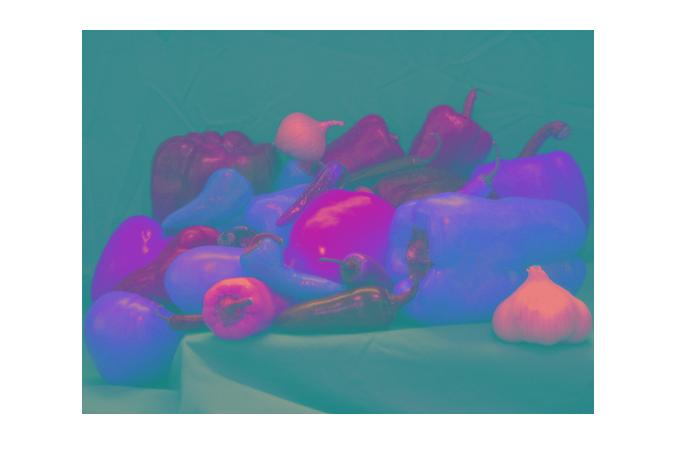
\includegraphics[width=0.45\linewidth]{question2/original image}
	}
	\subfigure[Luma Component]{
	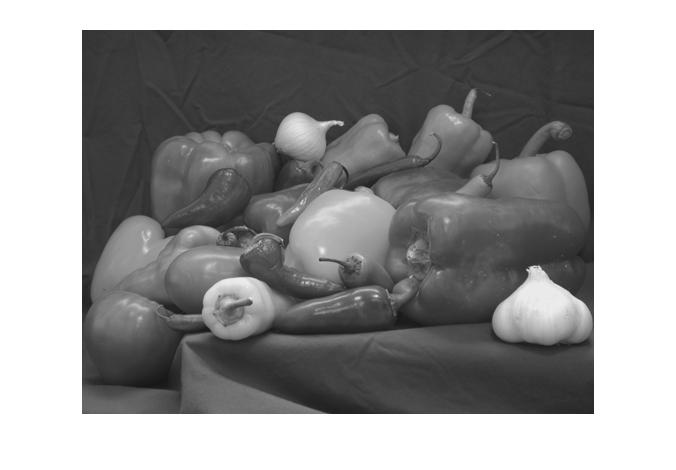
\includegraphics[width=0.45\linewidth]{question2/luma}
	}
	\subfigure[Cb Component]{
	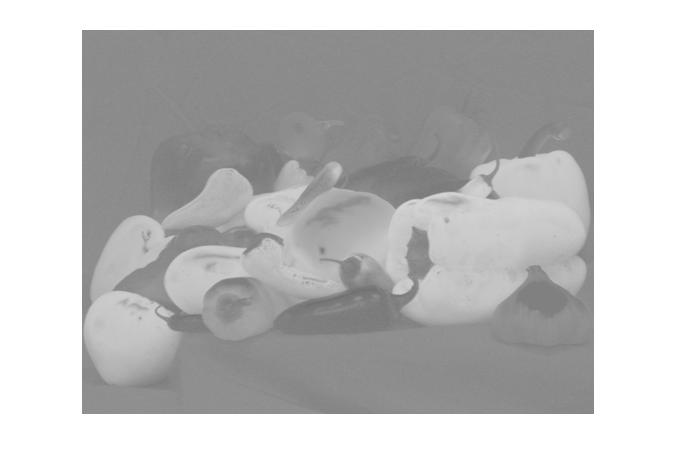
\includegraphics[width=0.45\linewidth]{question2/chroma_cb}
	}
	\subfigure[Cr Component]{
	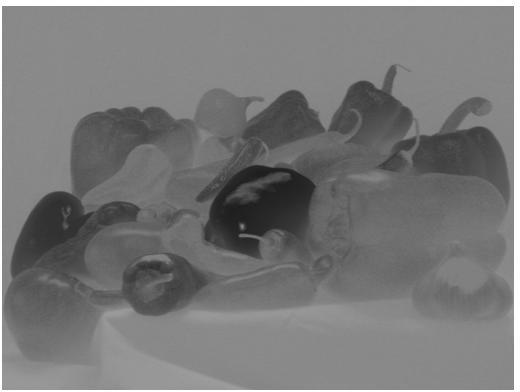
\includegraphics[width=0.45\linewidth]{question2/chroma_cr}
	}
	\subfigure[Chroma Subsampled]{
	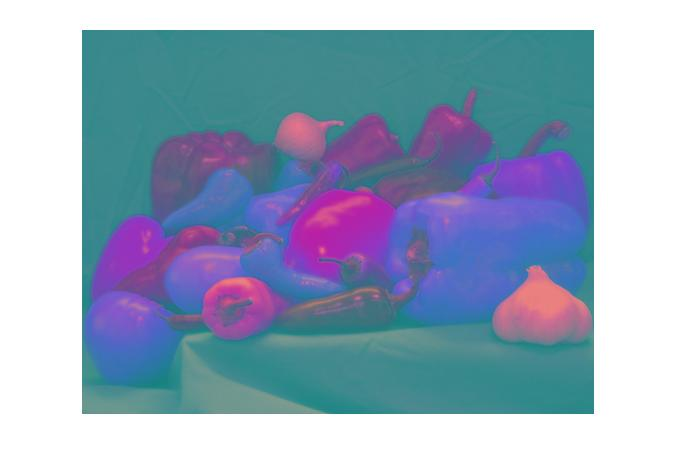
\includegraphics[width=0.45\linewidth]{question2/chroma_subsampled}
	}
	\subfigure[Luma Subsampled]{
	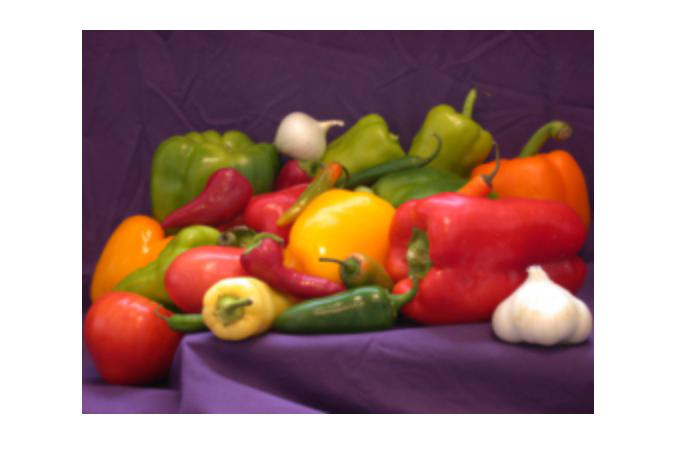
\includegraphics[width=0.45\linewidth]{question2/luma_subsampled}
	}
	\caption{Pepper image with YCrCb subsampling}
	\label{fig:noiseGeneration.toy}
\end{figure}
 

\subsection{Discussion questions}

\subsubsection{Describe the Cb and Cr channel images. Why do they appear this way?}
Cb is the blue difference chromatic component, and Cr is the red difference chromatic component. Cr has a higher image intensity at points where the original imagage contains high levels of red, and Cb has a higher intensity at points in the original image that contain high levels of blue.

\subsubsection{Compare the level of image detail in the Cb and Cr images with the Y channel image. Which contains
more ?ne details? What does that say about the luma (Y) and chroma (Cb and Cr) channels?}

The Y channel contains the most fine image detail. This means that the majority of the high frequency components are found in the luma channel.

\subsubsection{Compare the resulting image from chroma sub-sampling with the original image. How large are the
visual differences}
The visual differences are essentially non-existant.


\subsubsection{Based on the resulting image, what can you say about chroma sub-sampling and its effect on image
quality?}
Based on the subsampled images, it can be said that chroma sub-sampling (at least by a factor of two) has next to no impact on image quality, at least as far as the human eye can detect.


\subsubsection{Compare the resulting image from luma sub-sampling with the original image. How large are the
visual differences?}
The visual differences are more pronounced. The luma sub-sampled image is significantly blurrier than the original image.


\subsubsection{ Compare the resulting image from luma sub-sampling with the image produced using chroma subsampling. Which method performs better? Why}
Chroma subsampling performs significantly better than luma subsampling. 


\subsubsection{Based on the resulting image, what can you say about luma sub-sampling and its effect on image
quality}
Luma subsampling has a greater effect on image quality.
